\chapter{Решение проблемы возврата регенерированного урана в топливный цикл}

Далее будут представлены схемы, позволяющие решить поставленную в диссертационной работе задачу, отвечая всем сформулированным условиям для рассматриваемых составов регенерата, с различным исходным содержанием, что соответствует условиям многократного рецикла. Такие каскады позволяют добиться заданной цели возврата регенерата в топливный цикл -- одновременно выполнить ограничения на концентрации четных изотопов в продукте и обеспечить заданную пропорцию между исходным регенератом и продуктом.

\section{Схема двойного каскада с НОУ-разбавителем}

Развитием идеи двойного каскада является модификация в виде дополнительного использования в качестве разбавителя низкообогащенного урана, полученного из природного урана. Такая схема представлена на рис. \ref{p2left}. Принцип работы такой схемы опирается на идею <<пространственного>> разделения на легкую ($^{232,233,234}$U) и тяжелую фракции ($^{235,238}$U), предложенную в двойном каскаде, и заключается в следующем. 

\begin{figure}[ht]
    \centerfloat{
\includegraphics[scale=0.9]{cascades/p2left}}
    \caption{Схема модифицированного двойного каскада для обогащения регенерированного урана. Обозначения: $E$ -- поток регенерированного урана; $P_1$ -- поток отбора первого каскада, выступающий питанием второго каскада; $P_2$ -- поток отбора второго каскада; $W_1$ -- поток отвала первого каскада; $W_2$ -- поток тяжелой фракции (условный «отвал») второго каскада; $P_0$ -- поток НОУ-разбавителя; $P$ -- финальный продукт (товарный низкообогащенный уран (НОУ))}\label{p2left}
\end{figure}

В первом каскаде исходный материал обогащается по изотопам $^{232,233,234,235,236}$U, а во втором каскаде смесь делится на две фракции, так, чтобы в тяжелой фракции сконцентрировался продукт с пониженным содержанием $^{232,233,234}$U по отношению к питающей второй каскад смеси. Таким образом, в первом каскаде, на одном из концов, смесь обогащают по легким изотопы (в первую очередь $^{232,233,234,235}$U) в потоке $P_1$. Концентрацию $^{235}$U можно варьировать, однако целесообразно сохранять в диапазоне 5–20\%. Верхняя граница обусловлена ограничением на производство высокообогащенного урана \cite{brownOriginsSignificanceLimit2016}. Нижняя же граница диапазона обусловлена тем, что концентрация $^{235}$U в потоке $P_1$ должна быть выше требуемой к получению в потоке $W_2$ второго каскада, где этот поток будет обеднен по $^{235}$U. В легком же конце второго каскада сконцентрируются (будут доведены до более высокой концентрации, чем исходная) как изотопы $^{232,233,234}$U, так и $^{235}$U. Концентрация изотопа $^{235}$U в этом потоке ($P_2$) может доходить до значений, близких к 20\% и, если есть возможность добиться при этом улучшения целевых критериев производственного процесса, теоретически может быть доведена до 90\% при получении соответствующих разрешений. Следующим шагом к получению конечного НОУ является разбавление потока тяжелой фракции второго каскада $W_2$ сырьем, не содержащим искусственных изотопов урана для выполнения ограничений по $^{232}$U и $^{236}$U. В этом шаге и заключается отличие этой схемы от схемы-предшественника -- двойного каскада. Этот шаг и позволяет добиться требуемых пропорций вовлечения облученного топлива в воспроизводство свежего НОУ-топлива или, иными словами, выполнения условия полного использования регенерата. Для строгого соблюдения такой заранее определенной пропорции, вычисляется и пропорция подмешиваемого НОУ-разбавителя, легко рассчитываемая на основании параметров двойного каскада.

Предварительная оценка параметров каскадной схемы необходимых для получения НОУ-продукта требуемых качеств, показывает, что величина потока разбавителя $P_0$ должна в несколько раз превосходить по величине поток тяжелой фракции второго каскада $W_2$. Если бы в качестве разбавителя использовали природный уран, это ьы привело к снижению концентрации $^{235}$U в результирующей смеси ниже требуемой величины. Именно поэтому в схеме предусмотрен дополнительный каскад, нарабатывающий низкообогащенный уран в потоке $P_0$ из смесей природного (нереакторного) происхождения -- природного или обедненного урана.

Достоинствами рассматриваемой каскадной схемы являются:

\begin{enumerate}
    \item возможность полностью решить задачу возврата регенерированного урана в условиях многократного рецикла;
    \item частичное очищение регенерированного урана от четных изотопов $^{232,233,234}$U;
    \item обогащение даже загрязненного четными изотопами регенерированного урана, что делает схему применимой в условиях многократного рецикла.
    \item загрязнение меньшей доли разделительных мощностей четными изотопами, чем у разбавляющих каскадов, рассмотренных в главе 1, так как занятые под получение разбавителя остаются незагрязненными четными изотопами. Вдобавок, такой подход позволяет легко переориентировать ту часть разделительных мощностей, которая не соприкасалась с регенератом (поскольку разбавление происходит вне каскадов), на решение других задач;
\end{enumerate}

Основными недостатками рассматриваемой каскадной схемы, также как и остальных двойных каскадов, являются: 
\begin{enumerate}
    \item наличие «побочного» продукта в виде относительно небольшого (до 1–3\% от общей массы входящего потока регенерата) количество отхода -- загрязненной фракции, в которой сконцентрированы изотопы $^{232,233,234}$U, а также обогащен $^{235}$U;
    \item потери работы разделения при смешивании потоков с различным содержанием  $^{235}$U.

\end{enumerate}


\section{Схема двойного каскада с НОУ-разбавителем с возвратом потока $P_2$ в цикл}

В качестве модификации каскадной схемы, представленной на рис. \ref{P2utilizationRing}, в совместной публикации и патенте НИЯУ МИФИ и НИЦ «КИ» предложен способ, позволяющий вернуть поток $P_2$ в цикл для воспроизводства ядерного топлива (рис. \ref{p2left}) \cite{nevinicaToplivnyyCiklLegkovodnogo2019, nevinicaSposobIzotopnogoVosstanovleniya2019}. Принцип ее работы состоит в следующем.


\begin{figure}[ht]
    \centerfloat{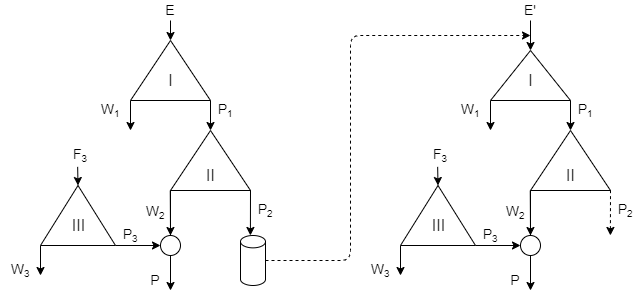
\includegraphics[scale=0.9]{cascades/P2utilizationRing}}
    \caption{Схема передачи загрязненной изотопом $^{232}$U фракции гексафторида урана в двойном каскаде от первой партии дообогащенного регенерированного урана к последующей. Обозначения: $E$ -- поток регенерированного урана; $P_1$ -- поток отбора первого каскада, выступающий питанием второго каскада; $P_2$ -- поток отбора второго каскада; $W_1$ -- поток отвала первого каскада; $W_2$ -- поток тяжелой фракции (условный «отвал») второго каскада; $P_0$ -- поток НОУ-разбавителя; $P$ -- финальный продукт (товарный низкообогащенный уран (НОУ)}\label{P2utilizationRing}
\end{figure}

Учитывая, что каскадная схема двойного каскада с НОУ-разбавителем (рис. \ref{p2left}) предназначена для обогащения регенерата с высоким накопившимся в ходе серии пройденых рециклов содержанием изотопа $^{232}$U, почему бы не использовать такую каскадную схему для вовлечения ранее полученного в потоке отбора второго каскада фракции $P_2$ загрязненной изотопом $^{232}$U. Выведенный ранее из системы гексафторида урана может быть перемешан с регенератом, полученным из следующей партии отработавшего топлива, то есть с составом более загрязненным изотопами $^{232,233,234,236}$U, чем исходно использовавшийся состав, побочным продуктом которого оказался этот $P_2$. Полученная таким образом в результате смешения $P_2$ предыдущего рецикла и регенерата очередного рецикла смесь будет отправлена на последующее обогащение (рис. \ref{P2utilizationRing}).

При использовании подобной схемы удастся полностью замкнуть топливный цикл по урану, а единственным отходом производства останется ОГФУ, образующийся в отвале первого каскада, который можно считать штатным отходом обогатительного производства с отработанными технологиями хранения и переработки. При этом после завершения производственного цикла останется невостребованным только тот объем обогащенного по изотопу $^{232}$U гексафторида урана (загрязненной фракции легкого конца второго каскада (рис. \ref{P2utilizationRing})), который будет образован после обогащения последней партии регенерата. Таким образом, предложенный подход к дообогащению регенерата урана позволяет организовать полный возврат регенерированного урана в топливный цикл в течение всего жизненного цикла задействованного урана.

При схожем наборе достоинств и недостатков схемы двойного каскада с НОУ-разбавителем с возвратом потока $P_2$ в цикл (рис. \ref{P2utilizationRing}) с предшественницей, не предусматривающей использование загрязненного потока (рис. \ref{p2left}), достоинством схемы с возвратом $P_2$ является более глубокая выработка потенциала делящегося $^{235}$U, накапливаемого совместно с изотопами $^{232,233,234}$U в загрязненной фракции второго каскада. Это позволяет добиваться меньших потерь $^{235}$ на всем жизненном цикле используемого урана.


\section{Схема тройного каскада с НОУ-разбавителем и дополнительным разбавителем потока $P_2$, возвращаемого в цикл}

Другим вариантом модификации каскадной схемы, представленной на (рис. \ref{p2left}) стала схема тройного каскада \cite{smirnovApplyingEnrichmentCapacities2018}. Принцип ее работы, наследуя заложенные в предшествующих схемах идеи, состоит в следующем дополнении.

\begin{figure}[ht]
    \centerfloat{
\includegraphics[scale=0.9]{cascades/p2_withDepU}}
    \caption{Тройной каскад для обогащения регенерированного урана.  Обозначения: $E$ -- поток регенерированного урана; $P_1$ -- поток отбора первого каскада, выступающий питанием второго каскада; $P_2$ -- поток отбора второго каскада; $W_1$ -- поток отвала первого каскада; $W_2$ -- поток тяжелой фракции (условный «отвал») второго каскада; $P_0$ -- поток НОУ-разбавителя; $P$ -- финальный продукт (товарный низкообогащенный уран (НОУ)), полученный смешиванием потоков $W_2$, $P_0$ и $P_3$, где $P_3$ -- отбор третьего каскада; $W_3$ -- отвал третьего каскада; .}\label{p2_withDepU}
\end{figure}

В реализации такой схемы поток легкой фракции второго каскада $P_2$ перемешивается со складским ОГФУ и направляется на последующее обогащение в третий каскад (рис. \ref{p2_withDepU}). Пропорцию смешивания $P_2$ с ОГФУ определяют исходя из возможности получить НОУ надлежащего качества при обогащении их смеси (оставаясь в рамках ограничений по четным изотопам). Остальные параметры схемы тройного каскада следует подбирать исходя из того, что финальный продукт будет получен смешиванием трех потоков: низкообогащенного <<чистого>> разбавителя $P_0$, тяжелой <<очищенной>> фракции $W_2$ второго каскада и, полученного при обогащении потока $P_2$ и обедненного урана, изотопного состава $P_3$. Управляющими параметрами являются: концентрации на выходах $P_1$ первого и $P_2$ второго каскадов, а также в потоке НОУ-разбавителя $P_0$. При детерминированной их комбинации обеспечивается соответствие предзаданному отношению масс конечного продукта и исходного регенерата, за счет чего выполняется условие полного возврата. При этом проблема высокоактивного отхода решается без выхода за пределы концентрации допустимой для обогащения регенерата (20\%). Также устраняется необходимость обращения с $P_2$, которое в схеме двойного каскада с НОУ-разбавителем с возвратом потока $P_2$ в цикл (рис. \ref{P2utilizationRing}) связано с его отложенным вовлечением из-за зависисмости от последующих поступлений на обогащение новых партий (последующих рециклов) регенерата.

Как результат, схема тройного каскада с НОУ-разбавителем и дополнительным разбавителем потока $P_2$, возвращаемого в цикл, позволяя в полноте решить поставленную задачу, не оставляет никакого нештатного отхода, требующего особых мер обращения. В конечном итоге образуется только штатный отход в виде отвалов $W_1$ и $W_3$ , процедуры обращения с которыми на разделительном производстве технологически отработаны. Если получить их смешением ($W_1$ и $W_3$) обедненный уран, он будет содержать изотопы $^{232,234}$U в количествах в десятки/сотни раз сниженных, относительно исходного регенерата. Следовательно, полученный в такой схеме обедненный уран может быть переведен в двуокись урана, например, при помощи установки «W-ЭХЗ». Отсутствие нештатных отходов, загрязненных четными изотопами и является отличительным достоинством рассмотренной схемы, тогда как недостатком выступают дополнительные потери работы разделения, возникающие при перемешивании потока $P_2$ и подмешиваемого к нему в качестве разбавителя ОГФУ. 













Для каждой из предложенных схем разработаны оригинальные методики расчета и оптимизации ее параметров по критерию минимума суммарного потока каскадной схемы, основанная на использовании современных методов условной оптимизации функций многих переменных. С использованием разработанных методик расчета и оптимизации предложенных каскадных схем продемонстрирована возможность их использования для обогащения регенерированного урана в условиях многократного рецикла на примере взятого из литературы изотопного состава регенерата урана с повышенным содержанием четных изотопов и отвечающего пятому рециклу в топливе ВВЭР.

-	схемы 1-3 пригодны для решения задачи обогащения регенерированного урана при описанных выше условиях в рамках многократного рецикла в топливе ВВЭР. При этом каждая из схем имеет собственные достоинства и недостатки. 

-	характерным недостатком схемы 1 является наличие отхода с высоким содержанием четных изотопов (на 1-2 порядка выше, чем пределы для товарного НОУ) и 235U (до 20\% или до 90\%, в зависимости от выбранного режима работы каскадной схемы). Одним из вариантом обращения с подобным отходом может стать его перемешивание с отвалом первого каскада при обогащении регенерата. Оценки показали, что в этом случае возможно получить обедненный уран с приемлемым содержанием 232U (не выше 5·10-7\%).
-	характерными недостатком схемы 2 является возврат значительной части четных изотопов на вход каскадной схемы;
-	характерным недостатком схемы 3 являются дополнительные затраты работы разделения по отношению к схемам 1 и 2, возникающие при обогащении разбавленного обедненным ураном отхода второго каскада схемы, загрязненного четными изотопами.

-	 Анализ эффективности предложенных каскадных схем с точки зрения потерь 235U показал, что перспективными вариантами для дальнейшей технико-экономической проработки являются каскадные схемы 1 и 3.



 схема 1 на каждом рецикле позволяет извлечь более 80\% от массы 235U из исходного регенерированного урана, поступившего на обогащение


Для выбора конкретного варианта каскадной схемы для организации производственного процесса, необходим детальный технико-экономический анализ каждой из схем на основе их интегральных показателей (расходные характеристики, затраты работы разделения и пр.) в контексте всей цепочки стадий ЯТЦ и с учетом возникающих в этой цепочке изменений при использовании регенерата урана по отношению к открытому топливному циклу. 

Помимо этого, необходима проработка технологических проблем каждой из схем, в частности, с точки зрения возможности эксплуатации и обслуживания оборудования в условиях работы с материалами, имеющими более высокую, чем природный уран удельную активность. Например, подобные условия возникают в «очистительных» каскадах, выделяющих в легкую фракции α-активные изотопы 232U и 234U. 
